%!TEX root =../../../course-notes.tex
% ^ leave for LaTeXTools build functionality
\begin{applicationActivities}
\begin{definition}
A  \term{first order ODE} is an equation involving (for a function \(y(x)\)) only  \(y'\), \(y\), and \(x\).
\vfill
We will most often deal with \term{explicit first order ODEs}, which can be written in the form \[y' = f(y,x)\] for some function \(f(y,x)\).
\end{definition}


\begin{activity}{5}
Consider the (explicit) first order ODE \[y' = y^2-x^2\].

\vfill

\begin{subactivity}
Compute \(y'\) at each of the points \( (1,1)\) , \((2,1)\), \((3, -2)\), and \( (4, -7) \).
\end{subactivity}
\begin{subactivity}

\end{subactivity}
Let \(y_0(x)\) be a solution that passes through the point \( (1,1) \).  What can you conclude about \( \lim _{x \rightarrow \infty} y_0(x) \) ?
\begin{enumerate}[(A)]
\item \( \lim _{x \rightarrow \infty} y_0(x) = -\infty \) 
\item \( \lim _{x \rightarrow \infty} y_0(x) \) is a finite number
\item \( \lim _{x \rightarrow \infty} y_0(x) = \infty \) 
\end{enumerate}
\end{activity}

\begin{definition}
These kinds of questions are easier to answer if we draw a \term{slope field} (sometimes called a \term{direction field}. 

To draw one, draw a small line segment or arrow with the correct slope at each point.

\begin{center}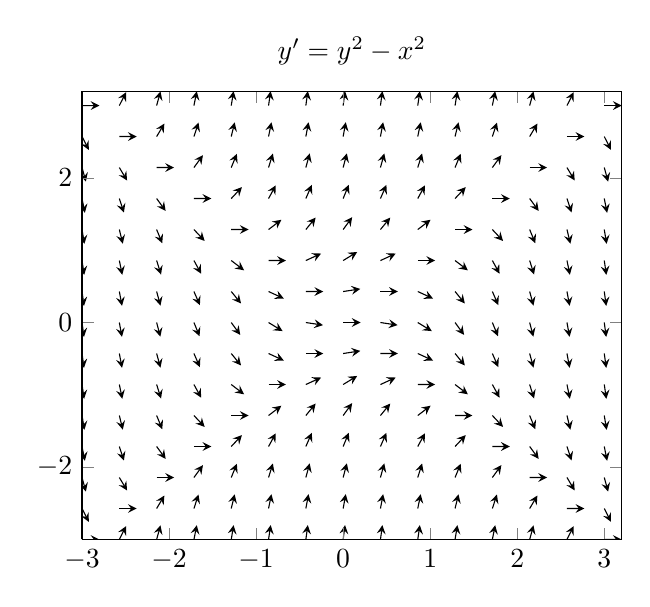
\begin{tikzpicture}
    \begin{axis}[
        title={\(y' = y^2-x^2 \)},
        domain=-3:3,
        view={0}{90},
        axis background/.style={fill=white},
    ]
        \addplot3[black,
            quiver={
             u={1/(sqrt(1 + (y^2 -x*x)^2))},
             v={(y^2 - x*x)/(sqrt(1 + (y^2 - x*x)^2))},
             scale arrows=0.2,
            },
            -stealth,samples=15]
                {exp(-x) - 1/2*sin(x) - 1/2*cos(x)};
    \end{axis}
\end{tikzpicture}\end{center}


\end{definition}

\begin{activity}{5}
\begin{center}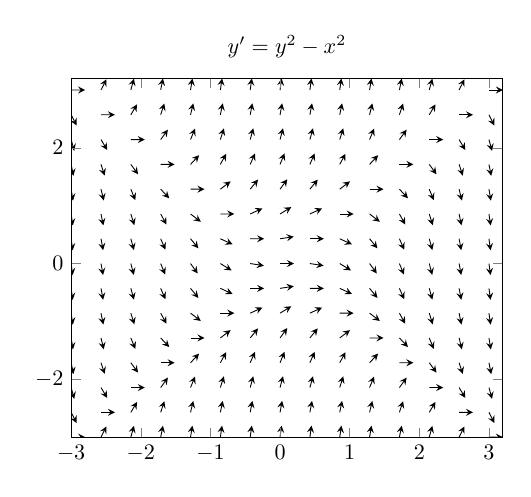
\begin{tikzpicture}[scale=0.8]
    \begin{axis}[
        title={\(y' = y^2-x^2 \)},
        domain=-3:3,
        view={0}{90},
        axis background/.style={fill=white},
    ]
        \addplot3[black,
            quiver={
             u={1/(sqrt(1 + (y^2 -x*x)^2))},
             v={(y^2 - x*x)/(sqrt(1 + (y^2 - x*x)^2))},
             scale arrows=0.2,
            },
            -stealth,samples=15]
                {exp(-x) - 1/2*sin(x) - 1/2*cos(x)};
    \end{axis}
\end{tikzpicture}\end{center}

Let \(y_1(x)\) be a solution that passes through the point \( (1,3) \).  What can you conclude about \( \lim _{x \rightarrow \infty} y_0(x) \) ?
\begin{enumerate}[(A)]
\item \( \lim _{x \rightarrow \infty} y_0(x) = -\infty \) 
\item \( \lim _{x \rightarrow \infty} y_0(x) \) is a finite number
\item \( \lim _{x \rightarrow \infty} y_0(x) = \infty \) 
\end{enumerate}

\end{activity}

\begin{activity}{15}
Consider the ODE \[y'=xy-x.\]
\begin{subactivity}
Draw a slope field for this ODE.
\end{subactivity}
\begin{subactivity}
Draw a solution that passes through the point (0,0).
\end{subactivity}
\begin{subactivity}
Draw a solution that passes through the point (-2,2).
\end{subactivity}
\end{activity}

\begin{observation}
\begin{center}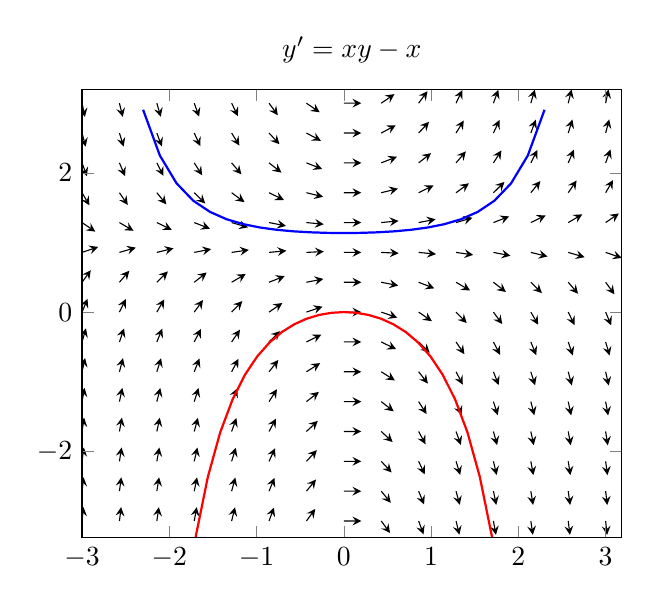
\begin{tikzpicture}
    \begin{axis}[
        title={\(y' = xy-x \)},
        domain=-3:3,
        view={0}{90},
        axis background/.style={fill=white},
    ]
        \addplot3[black,
            quiver={
             u={1/(sqrt(1 + (x*y-x)^2))},
             v={(x*y-x)/(sqrt(1 + (x*y-x)^2))},
             scale arrows=0.2,
            },
            -stealth,samples=15]
                {exp(-x) - 1/2*sin(x) - 1/2*cos(x)};
		\addplot[thick,red,domain=-1.7:1.7]{-e^(x^2/2)+1};
		\addplot[thick,blue,domain=-2.3:2.3]{e^(-2)*e^(x^2/2)+1};
    \end{axis}
\end{tikzpicture}\end{center}
\end{observation}

\begin{observation}
How can we solve \(y'=xy-x\) exactly?

\vfill
Notice \(xy-x=x(y-1)\), so we can write  \(y'=x(y-1)\).
\vfill
Write \[\frac{y'}{y-1} = x .\]

This is called a \term{separable} DE.
\end{observation}

\begin{observation}
Integrate both sides (and switch to Leibniz notation):
\[ \int \frac{1}{y-1} \frac{dy}{dx}\ dx = \int x\ dx .\]
The substitution rule (i.e. chain rule) says this is equivalent to 
\[ \int \frac{1}{y-1} dy = \int x\ dx .\]
Thus, \(\ln|y-1|=\frac{1}{2}x^2+c\).  Exponentiating, we have
\[|y-1|=e^{\frac{1}{2}x^2+c}=e^{\frac{1}{2}x^2}{e^c}=c_0 e^{\frac{1}{2}x^2}.\]

Allowing \(c_0\) to take on negative values, we can drop the absolute value sign, and obtain 
\[y=1+c_0e^{\frac{1}{2}x^2}.\]
\end{observation}

\begin{activity}{10}
Find the general solution to \[y'=xy+y.\]
\end{activity}

\begin{activity}{10}
Solve the IVP \[y'=\frac{x}{y}, y(0)=-1.\]
\end{activity}

\end{applicationActivities}
